\chapter{ПОДХОД МАШИННОГО ОБУЧЕНИЯ}

В этой главе будут даны основные определения, а также  сформулирована общая задача классификации.

Машинного обучение — это подраздел искусственного интелекта, находящийся на стыке статистики и компьютерных наук. Главная цель машинного обучения заключается в разработке методов, позволяющих строить математические модели, способные обучаться по прецедентам. Под обучением стоит понимать процесс аппроксимации заранее неизвестной функции по набору точек из её области определения и известных значений, полученных для каждой такой точки.

В нашем случае точки — это файлы формата .doc, а неизвестная функция отображает каждый такой файл во множество, состоящее из двух элементов {“вредоносный файл”, “безопасный файл”}.

Далее, мы более формально опишем, каким образом объекты  из реальной жизни можно рассматривать как точки, принадлежащие области определения неизвестной нам функции, и опишем подходы для извлечения зависимостей, c помощью которых в следующей главе будем решать задачи распознавания вредоносных программ.

\section{Обобщённая задача классификации}

Пусть $X$ — это множество объектов, а $Y$ — это множество классов и существует неизвестное нам отображение $F : X \to Y$, ставящее каждому объекту $x \in X$ в соответствие метку класса $y \in Y$.
Несмотря на то, что само отображение нам неизвестно, для некоторого набора элементов $\{ x_1, \dots , x_n \} \subset X$ мы можем получить значения $F$ в этих точках  $y_i = F(x_i)$, $i \in \{ 1, \dots, n \}$.
В такой постановке задачи набор пар $\{ (x_1, y_1), \dots, (x_i, y_i) \}$ называется обучающей выборкой и, имея такую выборку, нам необходимо построить функцию $F^*$, которая наилучшим образом приближает функцию $F$.
Конечно, мы хотим чтобы построенная функция $F^*$ не только возвращала метку $y = F^*(x)$ для точки $x$ из обучающей выборки, но и могла возвращать метку для новых, ранее неизвестных нам объектов, руководствуясь некоторым правилом.

Поиск $F^*$ можно свести к минимизации некоторого функционала $M(F^*, F)$, отражающего близость $F^*$ к $F$. В качестве $M$ можно взять, например, квадрат разности, тогда мы получим так называемый метод наименьших квадратов. Важно понимать, что уменьшение данной метрики на обучающей выборке не всегда приводит к уменьшению количества ошибок, совершаемых на новых объектах. Вопросы измерения качества классификации будут рассмотрены в следующих параграфах.

В некоторых случаях при использовании методов классификации нам важно знать не только конечную метку класса, но и степень уверенности в ней. В таком случае задачу классификации можно поставить следующим образом: существует неизвестное нам отображение $F : X \to Y$, ставящее каждому объекту из $X$ в соответствие метку класса из $Y$, необходимо по обучающей выборке $\{ (x_1, y_1), \dots, (x_i, y_i) \}$ получить функцию $F^* : X \to [0 \dots 1]^{|Y|}$, которая переводит объект в вектор вероятностей принадлежности к каждому из классов, и для любого $x \in X$ сумма $\sum_{i=1}^{|Y|} {F^*(x)}^{i} = 1$.

Получение значений приближенной функции $F^*$ предполагается производить на компьютере, поэтому алгоритм, который стоит за вычислением $F^*$, должен быть достаточно эффективным. 

Почти всегда функцию $F^*$ мы можем выбирать из некоторого параметризированного семейства функций, тогда задача поиска наилучшего приближения функции $F$ сводится к минимизации функционала $M(F^*, F)$ по вектору параметров, задающих $F^*$. Одним из подходов поиска параметров является градиентный спуск.

\section{Признаки объектов, матрица объект-признак}

Зачастую рассматриваемые нами объекты имеют довольно сложную структуру. Из-за этого могут появляться проблемы в формализации функций $F^*$ и $F$, введённых в предыдущем параграфе. Один из способов борьбы с такой проблемой — это перевод объекта в вектор формальных признаков.
Итак, пусть $x$ — элемент множества $X$. Введём набор функций $D_i$, отображающие $x$ в признаки $d_i$.

Признаки могут быть различных типов, например:
\begin{itemize}
\item бинарный, $d_i \in \{0, 1\}$
\item категориальный, $d_i$ принадлежит конечному множеству несравнимых между собой элементов
\item количественный, $d_i \in R$
\end{itemize}

Имея $\{D_1,…,D_m\}$, мы можем построить для каждого из объектов $\{x_1,…,x_n\}$ их признаковое описание. Таким образом, вместо множества объектов произвольной структуры мы будем оперировать матрицей $D$ размера $n$ на $m$.
Один из традиционных в статистике примеров такого подхода к решению задачи — это проблема классификации экземпляров цветка ириса.
В этой проблеме для каждого объекта выделяются 4 количественных признака:

\begin{itemize}
\item длина чашелистика
\item ширина чашелистика
\item длина лепестка
\item ширина лепестка
\end{itemize}

В качестве классов $y \in Y$ представлены три вида ирисов:
\begin{itemize}
\item Iris setosa
\item Iris versicolor
\item Iris virginica 
\end{itemize}


\begin{table}[ht]
\caption{Фрагмент матрицы объект-признак для задачи ирисов Фишера}
\label{tab_weight}
\centering
    \begin{tabular}{|c|c|c|c|c|}
    \hline Длина  & Ширина  & Длина  & Ширина  & Вид  \\
    чашелистика & чашелистика & лепестка & лепестка & ириса \\
    \hline 5.1 & 3 & 1.4 & 0.2 & setosa  \\
    \hline 7 & 3.2 & 4.7 & 1.4 & versicolor  \\
    \hline 6.3 & 3.3 & 6 & 2.5 & virginica  \\
    \hline
    \end{tabular}
\end{table}

В дальнейшем, при решении задачи классификации вредоносных объектов мы также перейдём от файлов к их признаковым описаниям и впоследствии к матрице объект-признак.
Имея на руках такую матрицу, мы можем применять большинство методов машинного обучения.

\section{Линейные модели классификации}

Одним из самых простых и распространенных методов построения классификаторов является логистическая регрессия.
Данный метод позволяет создавать модели предназначенные только для бинарной классификации.
Без ограничения общности будем считать, что множество классов равно $\{0, 1\}$.

Для того, чтобы построить классификатор, нам нужна только матрица объект-признак, введенная ранее. Мы подаём её на вход, а на выход получаем линейную модель, задаваемую набором чисел $\{a_0, a_1,…, a_m\}$, где $m$ это количество признаков у объектов. 

После этапа обучения мы можем предсказывать класс новых объектов следующим образом. Пусть $x$ — это новый объект, используя ранее введёные функции $\{D_1, \dots, D_m \}$, создаём признаковое описание $\{d_1,…,d_m\}$ элемента $x$. На этом шаге важно использовать те же самые функции \\ $D_i \in \{D_1, \dots, D_m \}$, с помощью которых была создана матрица объект-признак на этапе обучения.

Далее, мы вычисляем следующее выражение $ f \left( a_0 + \sum_{i=1}^{m} d_i * a_i \right)$, где $f \left( z \right) = \frac{1}{1 + e^{-z}}$. Значение данного выражения мы можем трактовать как вероятность принадлежности элемента к первому классу.

\begin{figure}[ht]
	\centering
    \begin{subfigure}[b]{1\textwidth}
    \centering
        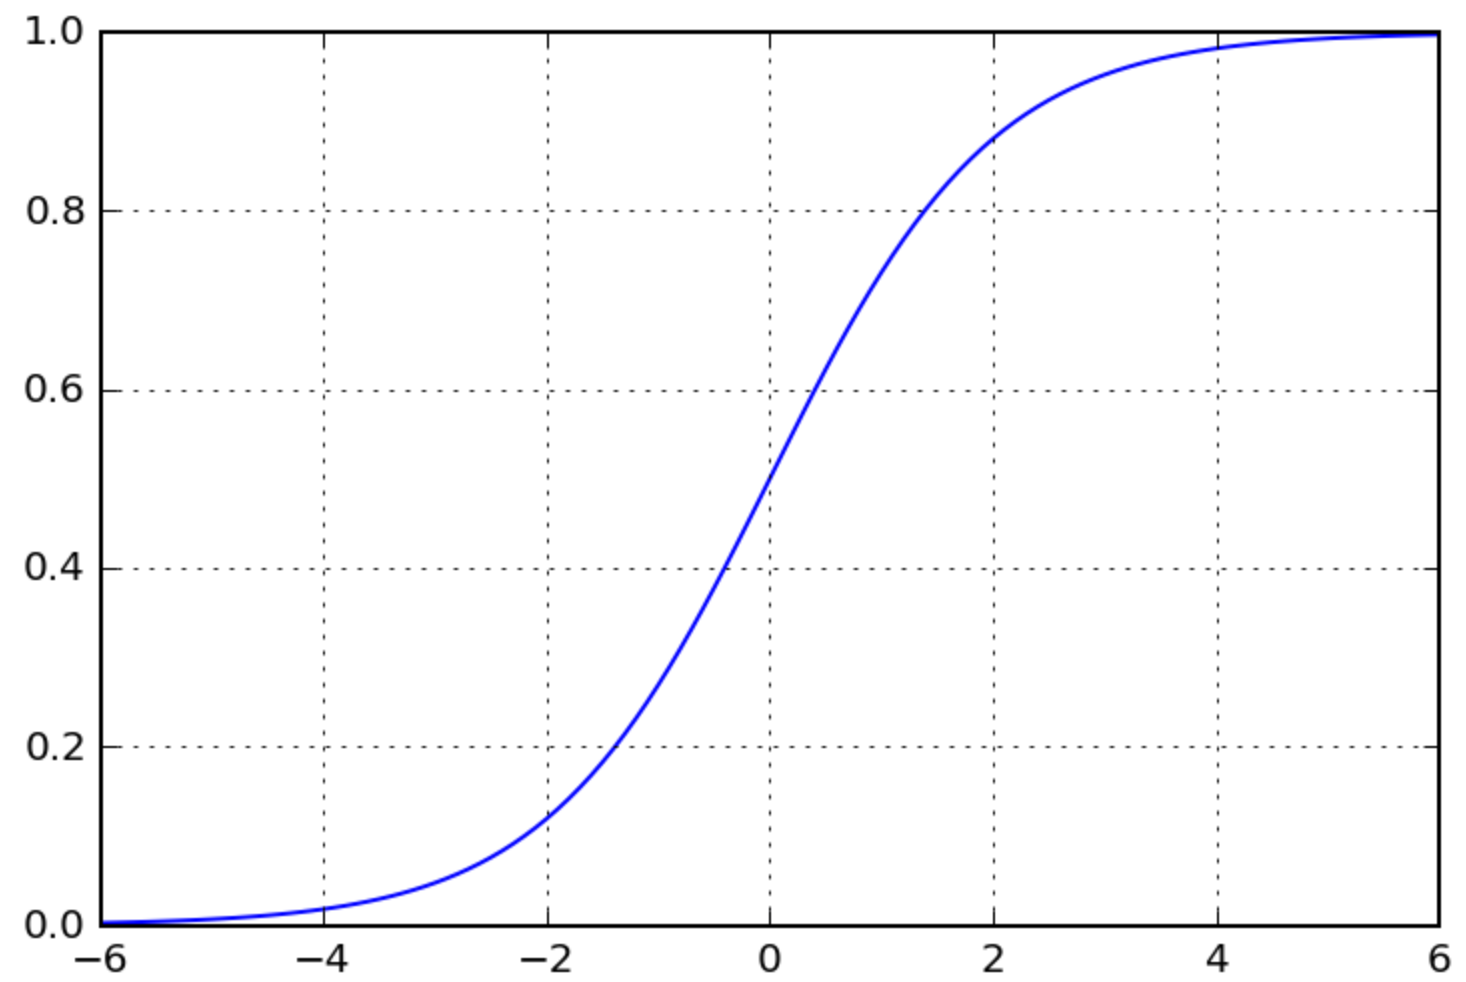
\includegraphics[scale=0.5]{pasted-image-15.png}
    \end{subfigure}
 
    \caption{График функции $f \left( z \right) = \frac{1}{1 + e^{-z}}$;}
    \label{fig_parsetree}
\end{figure}

Для поиска коэффициентов $\{a_0,…,a_m\}$, способствующих наилучшему приближению на обучающей выборке, существует множество эффективных методов. В дальнейшем мы будем использовать этот алгоритм для финального объединения результатов, полученных от большого набора других классификаторов. 

Данную модель можно интерпретировать следующим образом: модуль коэффициента при признаке под номером $i$ передаёт вес данного признака для итоговой оценки: чем он больше, тем важнее признак. Знак коэффициента отвечает за то, к какому классу мы будем отдавать предпочтение, если коэффициент отрицательный, то к классу “0”, если положительный, то, соответственно, классу “1”. Вычислив произведение вектора коэффициентов на вектор признаков, мы получаем число, которое необходимо сравнить с границей принятия решения $-a_0$. Если мы перешли эту границу, то метод будет отдавать предпочтение классу “1”, и, чем дальше данное число будет уходить за эту границу, тем будет больше вероятность принадлежности объекта к классу “1”. Данное рассуждение про физический смысл модели верно только, если все признаки объектов имеют одинаковый масштаб.

Конечно, логистическую регрессию можно использовать не только как способ объеденения других классификаторов. Ниже мы приводим пример решения задачи классификации цветков ириса. Для возможности визуалиации мы предварительно понизили размерность вектора признаков каждого объекта с четырёх признаков до двух. Для понижения размерности мы воспользовались методом главных компонент \cite{pca_book}\cite{pca_program}.

\begin{figure}[ht]
	\centering
    \begin{subfigure}[b]{1\textwidth}
    \centering
        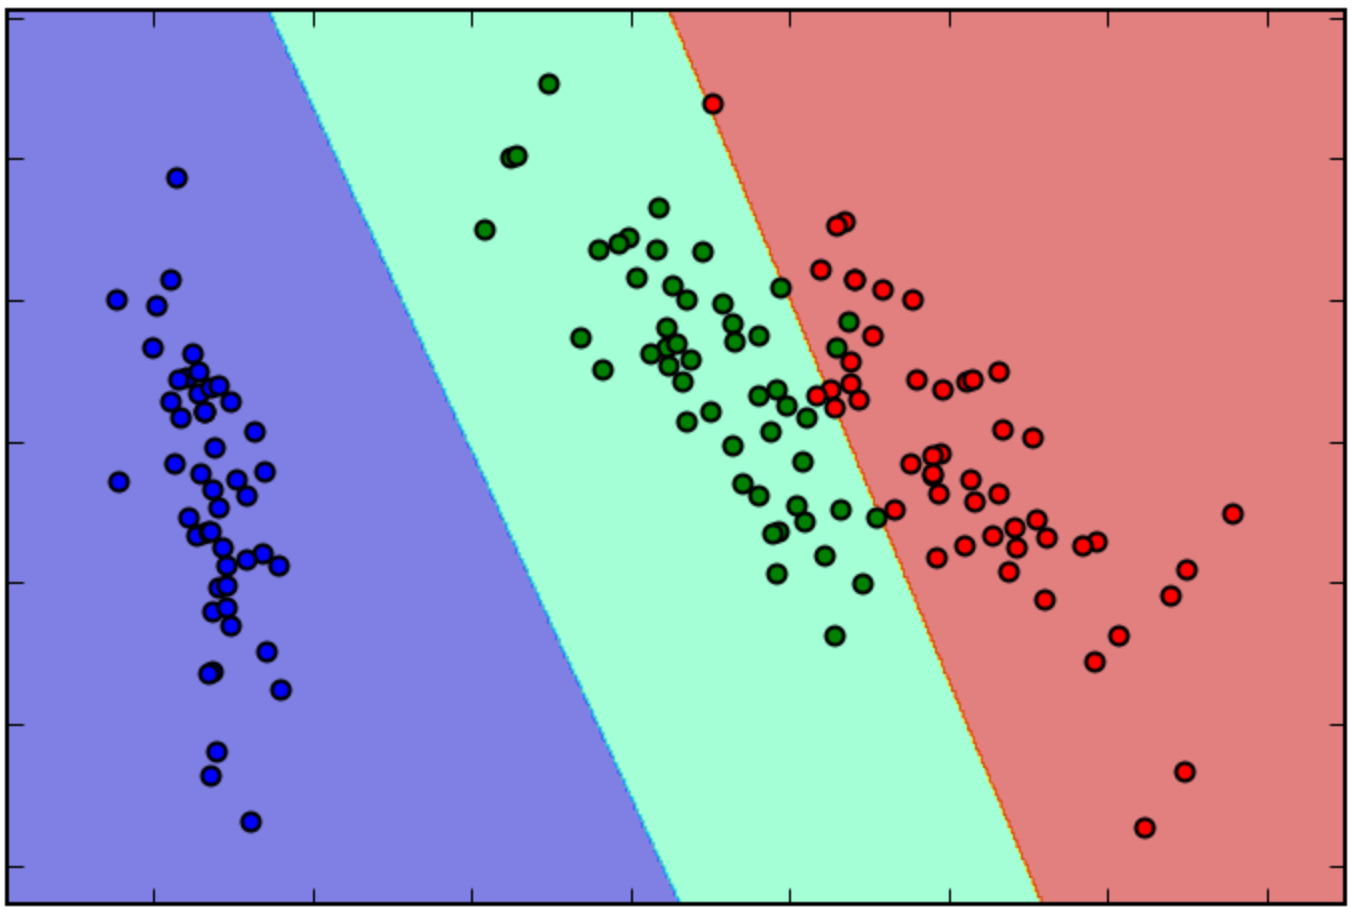
\includegraphics[scale=0.5]{pasted-image-19.png}        
    \end{subfigure}
 
    \caption{Ирисы Фишера, границы классов, полученные методом логистической регрессии;}
    \label{fig_parsetree}
\end{figure}

\section{Метрические алгоритмы классификации}

Существует другой подход к задаче классификации, базирующийся на следующем предположении: объекты из одного класса должны располагаться недалеко друг от друга относительно некоторой функции близости. Такой метод полезен в случаях, когда какой-то объект не описывается однозначно с помощью конечного числа признаков. Исходя из данного предположения, легко построить эвристический метод классификации, который называется метод K ближайших соседей.

Всё, что требуется от нас, это функция расстояния $F : X \times X \to R$, определённая для каждой пары объектов. Если рассмотреть одну из простых реализаций данного метода, то алгоритм классифицирующий новые объекты сводится к следующей последовательности действий.
Во-первых, мы сортируем элементы обучающей выборки в порядке возрастания  расстояния до нового объекта.
Во-вторых, мы выбираем K первых элементов отсортированной последовательности и подсчитываем, какой класс сколько раз встретился.
В итоге, новому объекту мы назначаем метку того класса, который встретился больше всего.

Кроме описаного варианта реализации также существуют более сложные, например, один из способов вводит такое понятие как вес объекта и позволяет оперировать им в процессе обучения, уменьшая вес элемента с увеличением его номера позиции в отсортированной выборке.

\newpage
\begin{figure}[ht]
	\centering
    \begin{subfigure}[b]{0.3\textwidth}
    \centering
        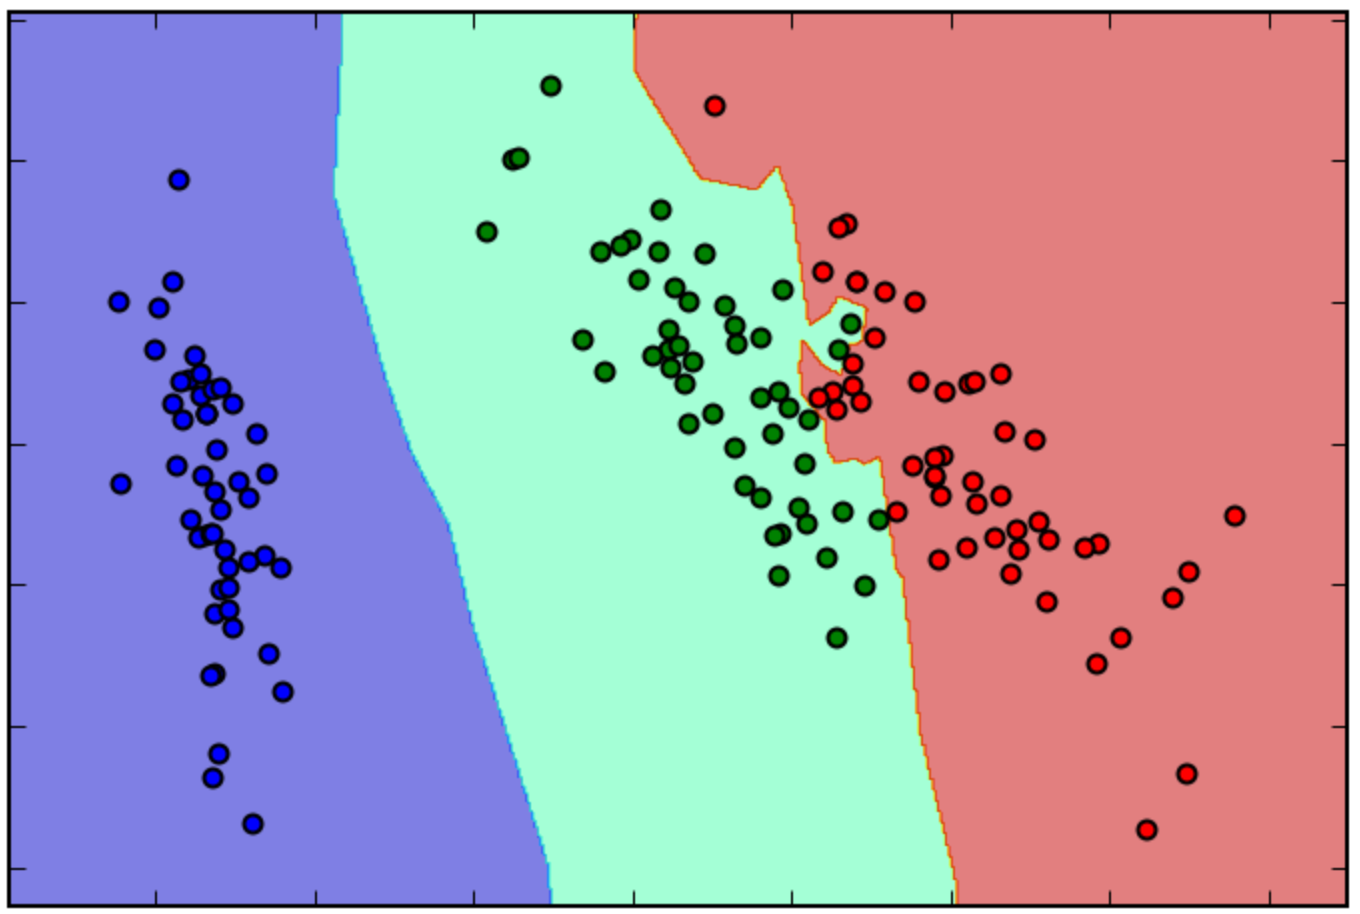
\includegraphics[scale=0.22]{pasted-image-21.png}
        \caption{}
    \end{subfigure}
 	\begin{subfigure}[b]{0.3\textwidth}
    \centering
        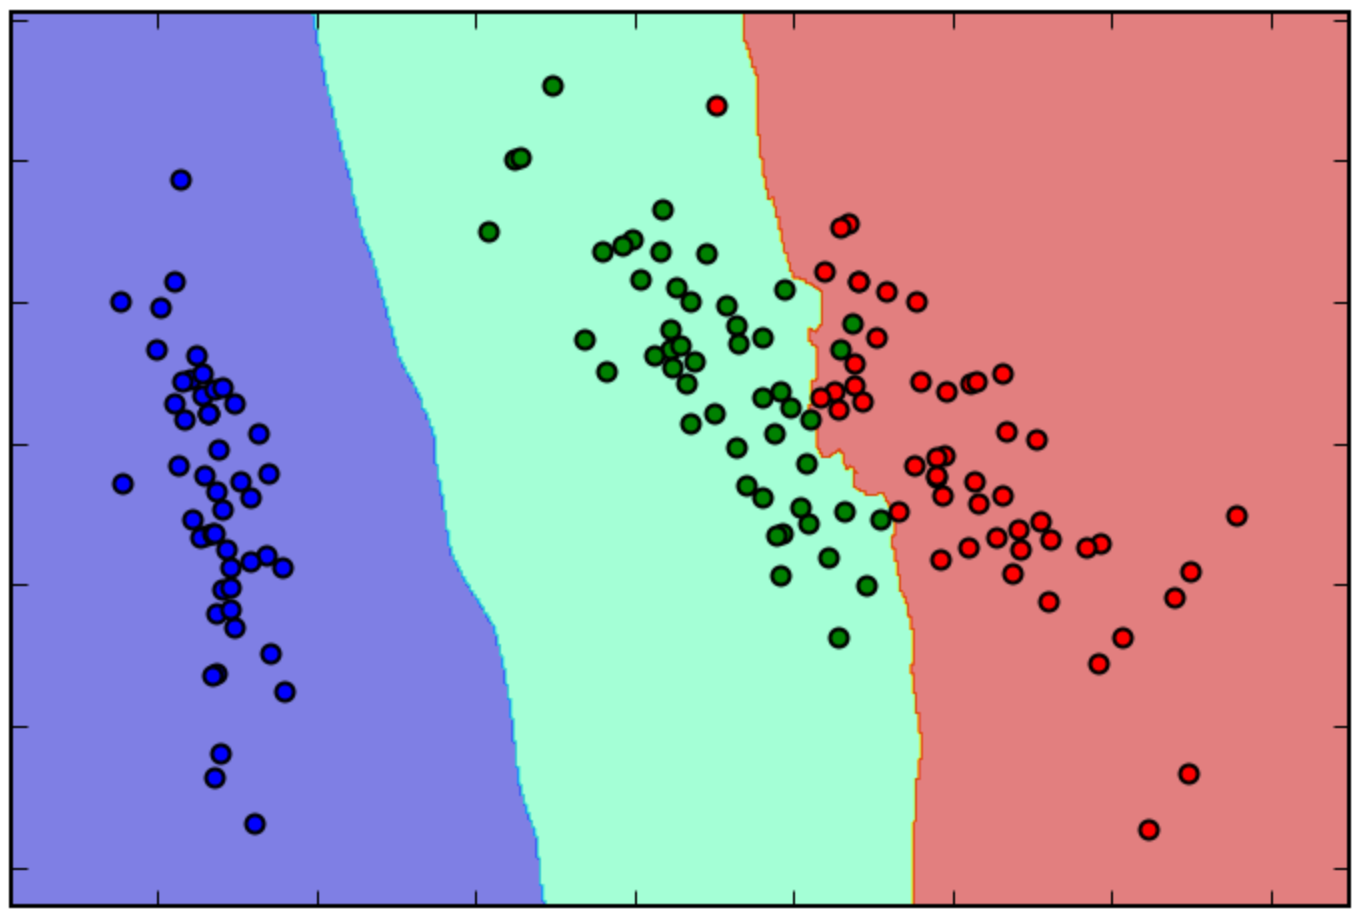
\includegraphics[scale=0.22]{pasted-image-23.png}
        \caption{}
    \end{subfigure}
    \begin{subfigure}[b]{0.3\textwidth}
    \centering
        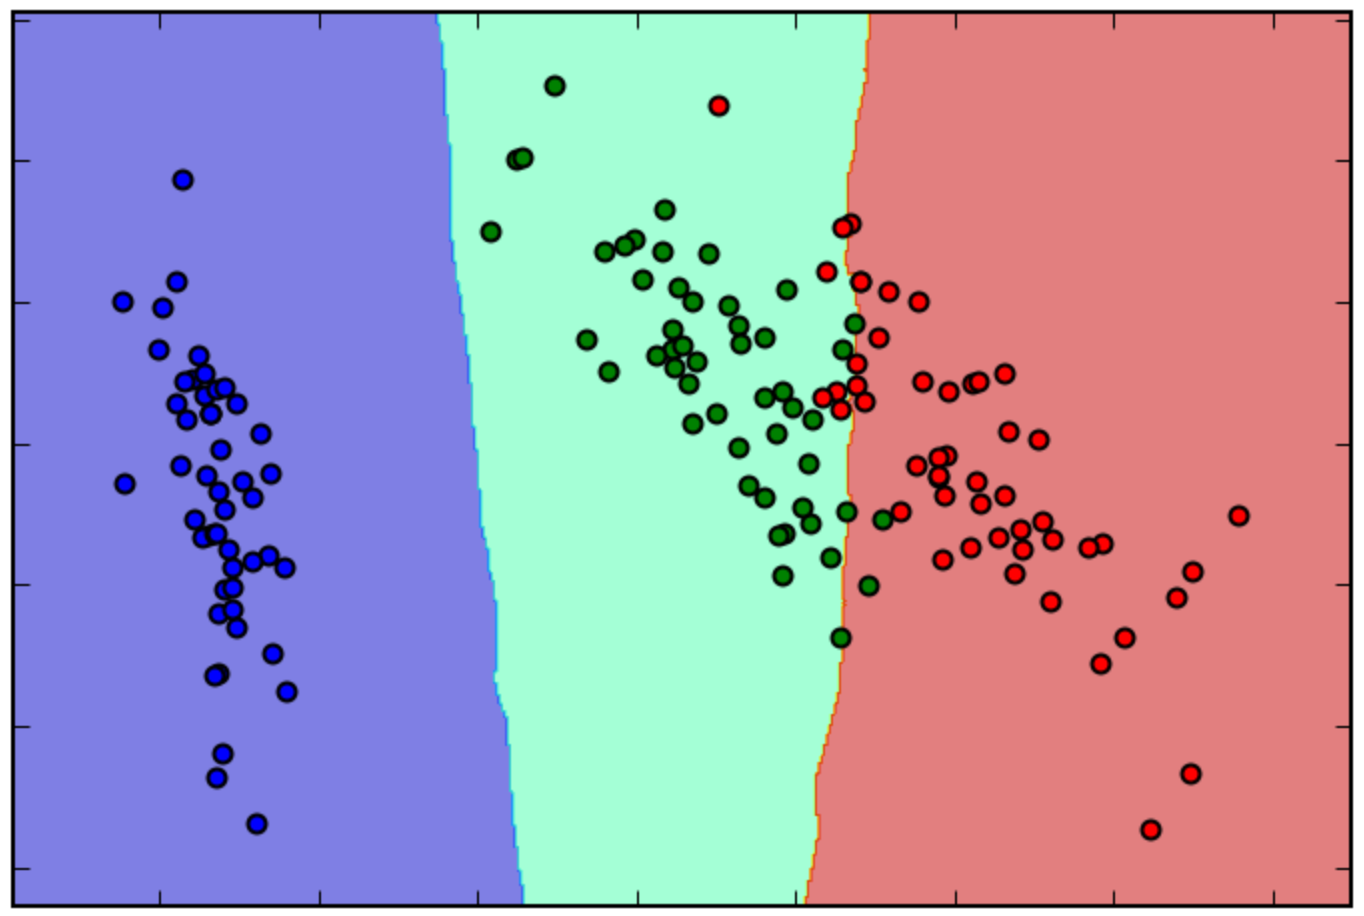
\includegraphics[scale=0.22]{pasted-image-25.png}
        \caption{}
    \end{subfigure}
    \caption{ Ирисы Фишера. Результат работы алгоритма K ближайших соседей; (a) Для K равного 1; (б) Для K равного 5; (в) Для K равного 50;}
    \label{fig_parsetree}
\end{figure}

Существует много готовых функций расстояний, например, если наш объект в обучающей выборке принадлежит пространству $R^n$, то в качестве функции расстояния можно взять Евклидову метрику.
Далее, когда нам будет необходимо сравнивать информацию о двух запущенных процессах, мы введём более сложную метрику.
На рисунке 3.3 визуально отображены границы классов в зависимости от числа соседей.
Количественные оценки качества каждого из вариантов будут представлены в следующем параграфе.

\section{Оценка качества классификации}

После того, как мы подобрали выборку, состоящую из рассматриваемых объектов, и построили по ним модель для классификации, наступает этап внедрения созданного метода в рабочий процесс. Во время работы для нас важно, как часто модель ошибается на новых объектах. Если ошибки будут возникать слишком часто, то польза от такого алгоритма будет поставлена под сомнение. 
Часто при оценке полученных моделей в машинном обучении прибегают к следующему способу: мы делим обучающую выборку на две части. Одну из частей мы по-прежнему будем использовать для обучения метода классификации, а вторую часть назовём тестовой выборкой и будем на ней проверять качество. Для каждого объекта из тестовой выборки мы с помощью нашего метода предсказываем метку класса и, далее, сравниваем полученный ответ с истинным. Истинный ответ нам известен, так как тестовая выборка является подмножеством изначальной обучающей выборки.

Имея на руках две метки класса, одну из которых мы получили от применения классификатора, мы можем применять огромное множество способов для оценки качества классификации. Один из способов, которым мы будем пользоваться в дальнейшем, основан на анализе матрицы ответов.

\begin{table}[ht]
\caption{Матрица возможных ответов классификатора}
\label{tab_weight}
\centering
    \begin{tabular}{|c|c|c|c|}
    \hline \multicolumn{2}{|c|}{} & \multicolumn{2}{c|}{Метка класса} \\
    \cline {2-4} & & 0 & 1 \\
   	\hline \multirow{2}{*}{Ответ классификатора} &  0 & TN & FN \\
   	\cline {2-4} & 1 & FP & TP \\
    \hline
    \end{tabular}
\end{table}


В данной матрице мы обозначили число в каждой ячейке заглавными латинскими буквами, рассмотрим что они означают:
\begin{itemize}
\item  TN, True Negative — количество объектов правильно классифицируемых как элементы класса “0”
\item  FP, False Positive — количество объектов, которое метод ошибочно отнёс к классу “0” (данный тип ошибок называется ошибками первого рода),
\item  FN, False Negative — количество объектов, которое метод ошибочно отнёс к классу “1” (данный тип ошибок называется ошибками второго рода),
\item  TP, True Positive — количество объектов, которые были правильно классифицированы и являются элементами класса “1”.
\end{itemize}
Через величины TN, FP, FN, TP вводятся промежуточные оценки классификации: полнота и точность.

\begin{figure}[ht]
\begin{align}
Recall &= \frac{TP}{TP + FN} \\[0.5cm]
Precision &= \frac{TP}{TP + FP}
\end{align}
\end{figure}

Значения полноты и точности принадлежат отрезку $[0 \dots 1]$. Значение полноты можно интерпретировать как вероятность того, что случайно выбранный элемент во время классификации будет отнесён к классу “1”, при условии, что он действительно принадлежит классу “1”. А значение точности — как вероятность того, что случайно выбранный элемент, отнесённый классификатором к классу “1”, действительно принадлежит классу “1”.

В случае задачи классификации вредоносных программ величина полноты предсказывает то, как часто мы будем пропускать вредоносные программы, а величина точности — насколько часто мы будем принимать хорошие программы за плохие.
В некоторых случаях удобнее иметь одну метрику для сравнения классификаторов вместо двух.
Для этого существует показатель, называющийся F-мерой, совмещающий в себе одновременно точность и полноту.

\begin{figure}[ht]
\begin{align}
F &= \frac{2 * Precision * Recall}{Precision + Recall}
\end{align}
\end{figure}

В дальнейшем мы будем сравнивать качество классификаторов именно по F-мере.
В момент отделения тестовой выборки возникает несколько проблем. Во-первых, мы можем поделить выборки таким образом, что одна из них получится смещённой по отношению к другой. В таком случае наша оценка классификатора окажется неверной. Во-вторых, мы теряем для использования в процессе обучения элементы, попавшие в тестовую выборку, и тем самым упускаем потенциальную возможность улучшить наш классификатор новыми данными. Для борьбы с этим можно использовать подход, имеющий название KFold. Мы делим обучающую выборку на N частей и последовательно используем в качестве тестовой выборки каждую из частей. После этого у нас будет N оценок классификатора, которые можно усреднить для получения финальной оценки. 
Также стоит упомянуть отдельный случай, когда N принимает значение равное длине выборки. То есть мы будем обучаться на всей выборке кроме одного объекта, а потом пытаться его предсказать. Данный метод имеет название Leave One Out или сокращённо — LOO. С помощью этого метода мы не сможем правильно посчитать точность, полноту и F-меру, но зато сможем понять по количеству ошибок насколько далёк наш классификатор от идеального. Этот метод проверки качества особо актуален в случае недостатка рассматриваемых объектов. 

\begin{table}[ht]
\caption{Сравнение метрик качеств для задачи ирисы Фишеры, взяты только два пересекающихся класса цветков}
\label{tab_weight}
\centering
    \begin{tabular}{|c|c|c|c|c|}
    \hline \multirow{3}{*}{\parbox{3.5cm}{Метод классификации}} & \multirow{3}{*}{Точность} & \multirow{3}{*}{Полнота} & \multirow{3}{*}{F-мера}  & \multirow{3}{*}{\parbox{3cm}{Количество ошибок при LOO}} \\
    & & & & \\
    & & & & \\    
    \hline \multirow{2}{*}{\parbox{3.5cm}{Логистическая регрессия}} & \multirow{2}{*}{0.96} & \multirow{2}{*}{1.0} & \multirow{2}{*}{0.97}  & \multirow{2}{*}{4} \\
    & & & & \\    
    \hline \multirow{2}{*}{\parbox{3.5cm}{1 ближайший сосед}} & \multirow{2}{*}{0.96} & \multirow{2}{*}{0.94} & \multirow{2}{*}{0.93}  & \multirow{2}{*}{6} \\
    & & & & \\ 
    \hline \multirow{2}{*}{\parbox{3.5cm}{5 ближайших соседа}} & \multirow{2}{*}{0.96} & \multirow{2}{*}{0.96} & \multirow{2}{*}{0.94}  & \multirow{2}{*}{5} \\
    & & & & \\ 
    \hline \multirow{2}{*}{\parbox{3.5cm}{50 ближайших соседей}} & \multirow{2}{*}{0.90} & \multirow{2}{*}{0.88} & \multirow{2}{*}{0.87}  & \multirow{2}{*}{9} \\
    & & & & \\     
    \hline
    \end{tabular}
\end{table}